\chapter{Experiments and Discussions}
For the quantification of how well our system works we need some measurements.
Unfortunately one of our input channels is not functioning (corresponding to the
D string), due to a hardware problems (not identified at the timing of writing this document),
hence it will be ignored. B string signal has DC noise,
due to resistor imprecisions (not fixed at the time of these experiments),
which limits the signal peak to peak value, and so it will have poor performance.
To make it simple our measurements will be based on mean and standard deviation.
A few measurements were proposed, as listed bellow and discussed on the following sections. 

\begin{itemize}
  \item Single Note Accuracy
  \item Whole Chord Accurracy (E and Am)
  \item Chromatic Scale Error
  \item Pluck Counting
\end{itemize}


\section{Single Note Accuracy}
This test is done by hitting a single note in a single string and checking if the right
frequency is being detected. The amount of detected notes will not be considered in this test.
The correct note and frequency are as in \autoref{single-note-expected-result}, chosen at random.
Considering the 8 first note detections, \autoref{single-note-accuracy} was drawn, showing
the detections for each algorithm. MacLeod's algorithm show more accurate results in this test.
The mean and standard deviation were also calculated, as in \autoref{single-note-result}.
MacLeod has a more accurate result, but YIN has a smaller standard deviation.
Our conclusion is that MacLeod has more accuracy and YIN has better consistency at single note
detection.

\begin{table}[htb]
  \begin{center}
    \ABNTEXreducedfont
    \caption[Single Note Expected Result]{Single Note Expected Result}
    \label{single-note-expected-result}
    \begin{tabular}{c | c | c}
      \hline
      String & Frequency(Hz) & Note (name and number)\\
      \hline \hline
      E (6) & 493.9 & B4 (71) \\ \hline
      A (5) & 370 & Gb4 (66) \\ \hline
      G (3) & 293.7 & D4 (62) \\ \hline
      B (2) & 164.8 & E3 (52) \\ \hline
      e (1) & 123.5 & B2 (47) \\ \hline
    \end{tabular}
    \legend{Source: authors}
  \end{center}
\end{table}

\begin{table}[htb]
  \begin{center}
    \ABNTEXreducedfont
    \caption[Single Note Result]{Single Note Result}
    \label{single-note-result}
    \begin{tabular}{c | c | c | c | c}
      \hline
      String & MacLeod Mean (Hz) & MacLeod Standard Deviation & YIN Mean (Hz) & YIN Standard Deviation\\
      \hline \hline
      E (6) & 495.27 & 0.04 & 489.81 & 0.012 \\ \hline
      A (5) & 379.00 & 0.13 & 368.09 & 1.27 \\ \hline
      G (3) & 298.28 & 1.59 & 301.43 & 0.60 \\ \hline
      B (2) & 167.00 & 0.04 & 164.01 & 0.08 \\ \hline
      e (1) & 124.47 & 0.16 & 121.13 & 0 \\ \hline
    \end{tabular}
    \legend{Source: authors}
  \end{center}
\end{table}


\begin{figure}[!htpb]
  \centering
  \caption{Strings Single Note Accuracy}
  \label{single-note-accuracy}
  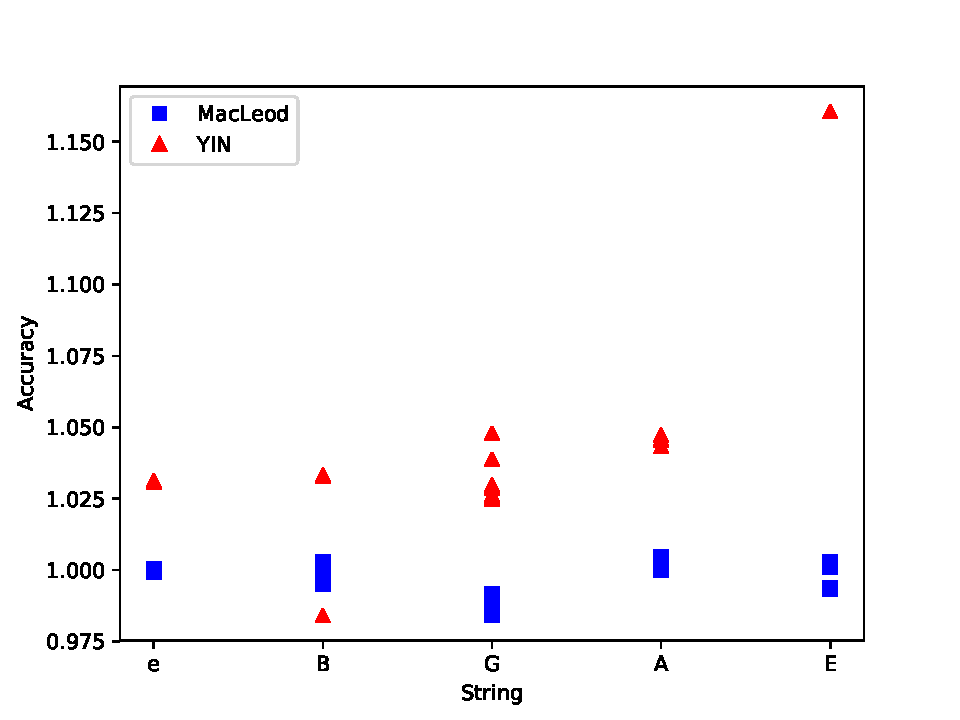
\includegraphics[scale=0.85]{images/measurements/single-note-acc-2}
  \legend{Source: Authors}
\end{figure}

\section{Chord Detection}
This test was done to detect notes playing simultaneously at multiple strings.
Two chords were test E major and A minor (Am). The E chord has it's lower note on
the twelfth fret, to cut off very low frequencies. The Am chord has it's lower note
on the fifth fret, and so lower frequencies.
The error rate and standard deviation were calculated for both cases. The error rate is given by
\autoref{chord-accuracy-equation}. The result can be seen at \autoref{e-chord-error} and \autoref{am-chord-error}, where the
error is given in percentage but the standard deviation in absolute values.
Our conclusion is that YIN has better accuracy, except at low frequencies where it
has huge errors rate.

\begin{equation}
  \label{chord-accuracy-equation}
  Accuracy = \frac{Mean - Expected\ Value}{Expected\ Value} = \frac{\sum x}{Length * Expected\ Value} -1
\end{equation}

\begin{figure}[!htpb]
  \centering
  \caption{Am Chord Error}
  \label{am-chord-error}
  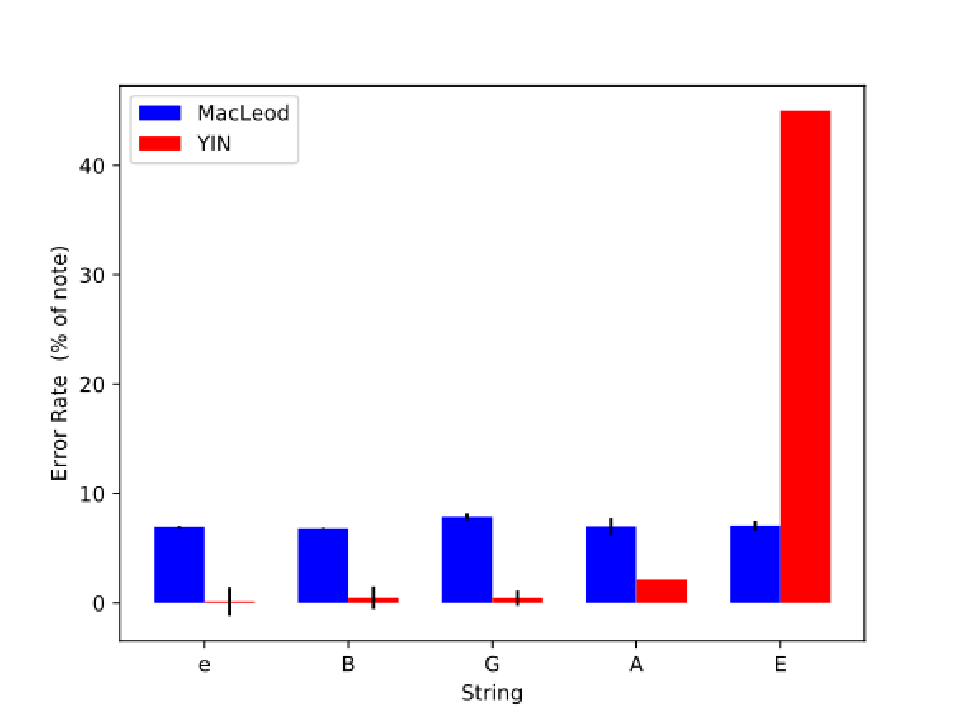
\includegraphics[scale=0.85]{images/measurements/am-chord-error}
  \legend{Source: Authors}
\end{figure}

\begin{figure}[!htpb]
  \centering
  \caption{E Chord Error}
  \label{e-chord-error}
  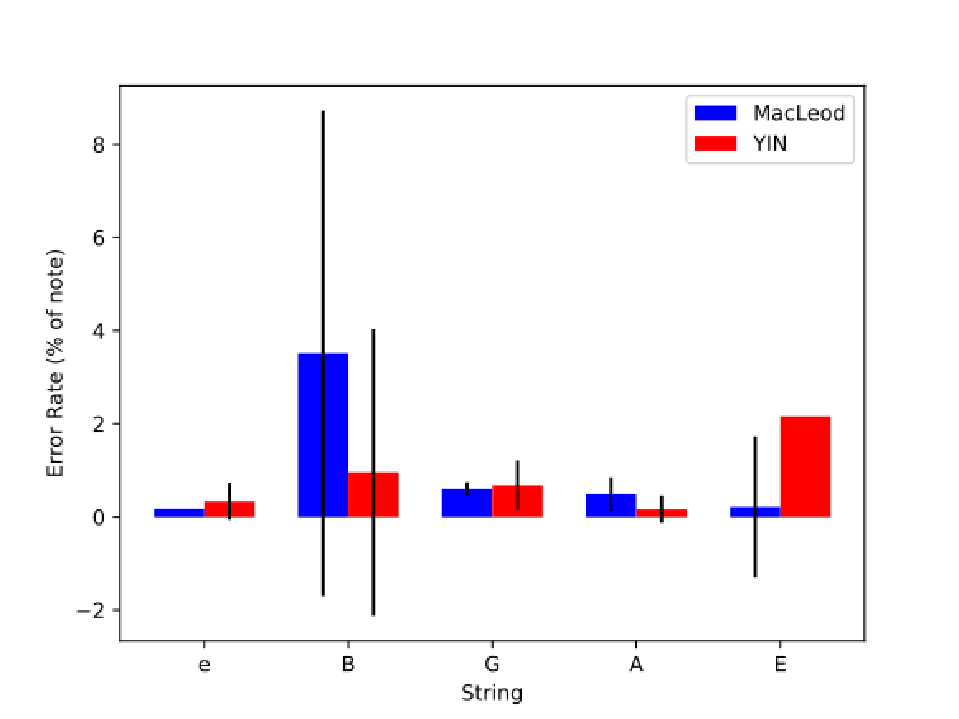
\includegraphics[scale=0.85]{images/measurements/e-chord-error}
  \legend{Source: Authors}
\end{figure}

\section{Chromatic Scale Error}
This is the last note detection experiment and it will try to test the detection
of notes over time. Each string was played separately by plucking 5 consecutive
notes (e.g. A, A\#, B, C and C\#) at the speed of approximately 4 notes/s, which
is a medium speed for guitar playing. To avoid pluck miss-detections in this test, repeated notes
are grouped into a single detection. The measurements were then compared with the
expected output, and any miss-detection counted. This test was repeated five times,
and the mean was taken as the error rate, calculated by dividing the number of 
errors by the total number of distinct detected notes. The result in \autoref{chromatic-scale-error}
show that MacLeod has better precision when the time dimension comes to be.

\begin{figure}[!htpb]
  \centering
  \caption{Chromatic Scale Error}
  \label{chromatic-scale-error}
  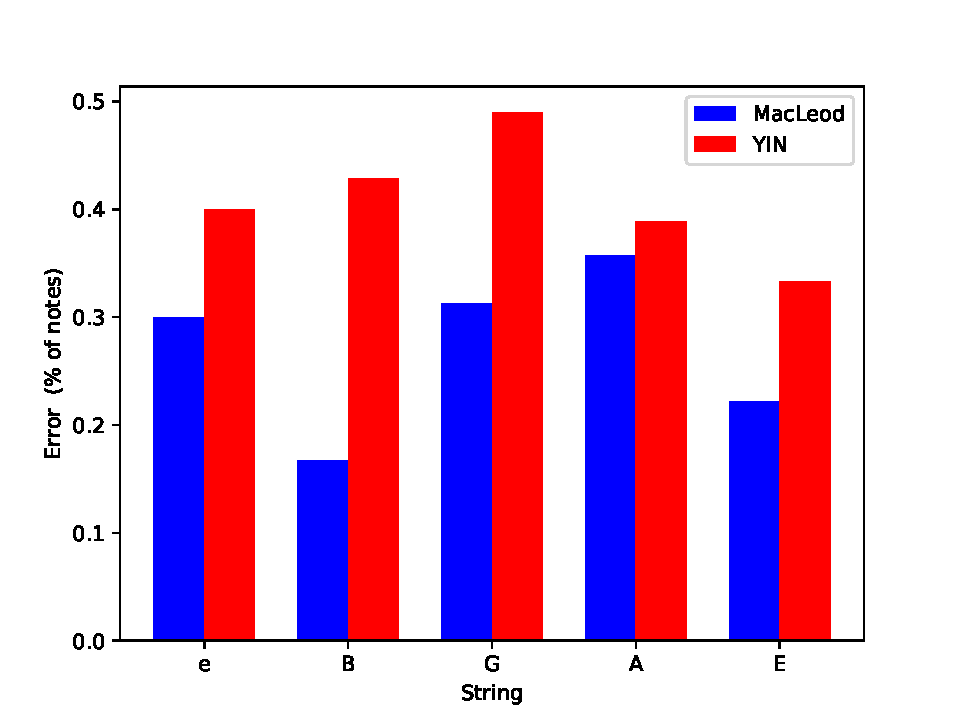
\includegraphics[scale=0.85]{images/measurements/chromatic-scale-error}
  \legend{Source: Authors}
\end{figure}

\section{Pluck Counting}
At last an experiment was made to test the amplitude detection of the same note.
By playing a single note 20 times in a row (approximately 4 notes/s again) and counting
how many notes were actually detected, for each string, and then taking the mean of all strings.
The result is as in \autoref{pluck-hits-counting}. The results are close, and the conclusion
is that simple amplitude detection by taking the AC mean of the current window is not enough
to correctly detect amplitude changes. At least not with the current selected parameters.

\begin{table}[htb]
  \begin{center}
    \ABNTEXreducedfont
    \caption[Pluck Hits Counting]{Pluck Hits Counting}
    \label{pluck-hits-counting}
    \begin{tabular}{c|c|c}
      \hline
      Correct Value & MacLeod & YIN \\
      \hline
      20 & 29.2 & 27 \\
      \hline
    \end{tabular}
    \legend{Source: authors}
  \end{center}
\end{table}

\section{Discussions}
Strings Single Note Accuracy test gave satisfactory results (\autoref{single-note-accuracy}).
This limited the channel gain which ultimately made this
channel results lower than the others. The same analysis is true for
all other experiments.

Both the chord detection experiments (\autoref{am-chord-error}, \autoref{e-chord-error}) gave reasonable results, but they
show our system still has lots of room for improvement. The exception is for
the E string error on the Am chord using the YIN algorithm. The reason
for this is that YIN is not working well for low frequency notes, because
it still needs a greater period (samples) for analysis, which is not currently
possible due to processing time limitations - but a solution is proposed at
the next chapter.

The chromatic scale results (\autoref{chromatic-scale-error}) show that our system is not working well along time.
By using a small period of measurement (so it can run at real-time) the range
where a note is changing to the next one is misread as an incorrect result.
This is a big problem for music annotation, but has the same solution as above,
which needs performance improvement.

The last test (\autoref{pluck-hits-counting}) also shows our time related issues,
that, although being natural, still need to be dealt with, for the same reason above, transitions
through time that need a larger sample period to work well, also a better algorithm to detect
amplitude changes. The plucking errors are due to the amplitude detection.
